
\section*{Über die Fakultät}

\begin{wrapfigure}{l}{3cm}
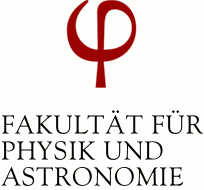
\includegraphics[width=3cm]{logo.png}
\end{wrapfigure}



Nach zahlreichen ZaPFen hast du es nun endlich in deinem Leben zu etwas gebracht. Du bist an der prestigeträchtigen Heidelberger \textbf{Fakultät für Physik und Astronomie} angekommen. Da bist du aber nicht der*die Einzige.
Aktuell sind hier ca 2000 Studis in der Physik eingeschrieben.
Zum Glück ist unsere Fakultät mit einer Vielzahl Einrichtungen und einer großen Bandbreite an Vertiefungsmöglichkeiten gut aufgestellt.\\

\begin{wrapfigure}{r}{4cm}
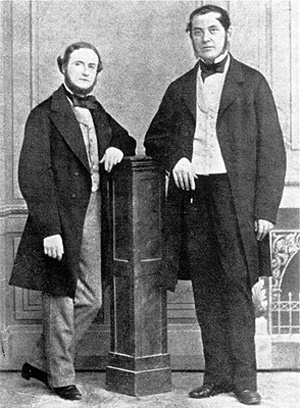
\includegraphics[width=4cm]{kirchhoff.JPG}
\end{wrapfigure}

Das \textbf{Kirchhoff-Institut für Physik (KIP)} beherbergt neben den für dich als Zapfika relevanten Hörsäalen und Seminarräumen experimentell tätige Forschungsgruppen im Bereich klassischer Komplexer System (Neuromorphe Hardware, Biophysik, Nanotechnik), Quantensysteme (von ultrakalten Quantengasen bis hin zur Festkörperphysik) sowie zu Fundamentalen Teilchen und Wechselwirkungen, letzteres zur Entwicklung von Detektoren und Kalorimetern in enger Zusammenarbeit mit Forschungsstätten wie dem CERN und der GSI.

Angrenzend an das KIP befindet sich im Klaus-Tschira-Gebäude das \textbf{Physikalische Institut (PI)}, wo du auch im goldenen Käfig in den Genuss unseres ewigen (endgeilen) Frühstücks kommen wirst. Hier forscht man zu Niederenergie- und Hochenergieteilchenphysik, Theorie und Experiment von komplexen Quantensystemen sowie der Schwerionenphysik. Im Erdgeschoss haben viele Studis im Anfängerpraktikum den Spaß ihres Lebens.

Benachbart an das PI liegt das 2017 eröffnete \textbf{Center for Advanced Materials (CAM)} einer interdisziplinären Forschungsstätte für die Erforschung und Herstellung sogenannter neuer Materialien, wie zum Beispiel im Gebiet der organischen Elektronik.
In dem aktuell noch in Bau befindlichen Gebäude neben dem CAM wird das Human Brain Project Platz finden. 

Gegenüber des CAMs liegt das \textbf{Institut für Umweltphysik (IUP)}, das erste seiner Art in Deutschland, von der Atmosphäre über den Ozean hin zu Böden, Gewässern und Gletschern widmet man sich unserer Umwelt hinsichtlich ihrer Vergangenheit, Gegenwart und zukünftigen Entwicklung. Im Bereich der Bildverarbeitung und des maschinellen Lernens bestehen enge Verbingungen zur Informatik, insbesondere mit dem Heidelberg Collaboratory for Image Processing (HCI).

\begin{wrapfigure}{r}{4cm}
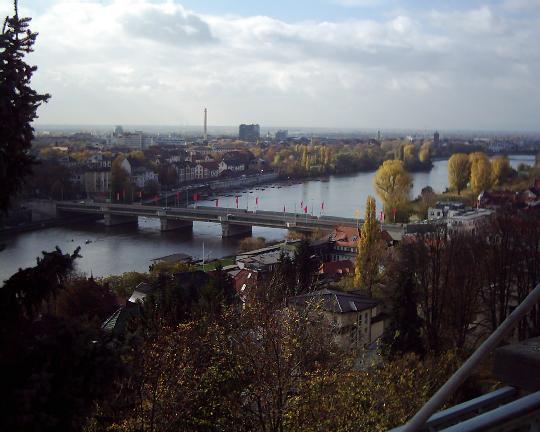
\includegraphics[width=4cm]{aussicht.jpg}
\end{wrapfigure}

Auch die Theorie kommt bei uns nicht zu kurz und bietet einige Verlockungen an. Am Philosophenweg 12, dem ehemaligen Sitz des physikalischen Instituts und in zwei Villen (Hausnummer 16 und 19) gehen die Wissenschaftler*innen des \textbf{Instituts für Theoretische Physik (ITP)} den grundlegendsten Fragen unserer Zeit nach. Teilchenphysik, Stringtheorie, Kosmologie, Quantendynamik, theoretische Festkörper- und Biophysik, das Spektrum könnte kaum breiter sein. Von wegen graue Theorie, bei dieser herrlichen, inspirierenden Aussicht entfaltet sich für die Theoretiker*innen in Heidelberg das Grün des Lebens goldner Baum in voller Pracht.
\begin{wrapfigure}{l}{3cm}

\includegraphics[width=3cm]{zah_logo.jpg}
\end{wrapfigure}

Nun mag der aufmerksamen Leserin vielleicht aufgefallen sein, dass sich im Namen unserer Fakultät noch ein weiteres großes Betätigungsfeld der Physik verbirgt, die Astronomie. Von der Theorie bis hin zur direkten Observation, diese hat in Heidelberg viele Facetten.
Das \textbf{Zentrum für Astronomie der Universität Heidelberg (ZAH)} vereint das
Astronomische Rechen-Institut (ARI), die Landessternwarte Königstuhl (LSW) und das Institut für Theoretische Astrophysik (ITA) und liegt über das Stadtgebiet verstreut. 

Weitere Betätigungsmöglichkeiten für Physiker*innen bieten das zentrale Institut für Technische Informatik (ZITI), das Physikalisch-Chemische Institut (PCI) und das Interdisziplinäre Zentrum für wissenschaftliches Rechnen (IWR).

All diese Institute und Forschungsbereiche haben auch meist eigene Colloquia, hervorzuheben ist hier das Größte und Bekannteste, das physikalische Colloquium. Dieses findet immer Freitags statt, auch während der ZaPF, 17 Uhr ct im Hörsaal 1 in der 308. Nach dem Vortrag laden Wein und Bretzeln zum sinnieren über die neugewonnenen Erkenntnisse ein.

Heidelberg kann auch einige externe Einrichtungen mit Physikbezug aufweisen, wie die drei \textbf{Max-Planck-Institute} für Kernphysik, Astronomie und medizinische Forschung. Zudem bietet sich das European Molecular Biology Laboratory (EMBL), das deutsche Krebsforschungszentrum (DKFZ) sowie das Heidelberger Institut für theoretische Studien (HITS) Gelegenheit für Projektpraktika und Forschungsarbeiten.

Promotionsstudierende haben zudem die Möglichkeit in einer der Graduiertenschulen unterzukommen. 
Die im Rahmen der Exzellenzinitiative entstande \textbf{Heidelberg Graduate School of Fundamental Physics (HGSFP)} fördert Promovent*innen von  allen physikalischen Vertiefungsrichtungen, um durch das Erkennen der Verbindungen zwischen den einzelnen Fachrichtungen das große Ganze sichtbar zu machen.
Desweiteren existiert die Heidelberg Graduate School of Mathematical and Computational Methods for the Sciencs (HGS MathComp) zur Förderung von Promovierenden und Post-Docs im weiten Feld des Scientific Computings.\\

%BILDQUELLEN: 
%http://www.physik.uni-heidelberg.de/images/logo_physik_de.gif 
%https://commons.wikimedia.org/wiki/File:Kirchhoff-Institut_f%C3%BCr_Physik_Uni_Heidelberg.JPG
%https://www.thphys.uni-heidelberg.de/images/wetzel/100V1310.b/DSCI0001.JPG
%http://www.ita.uni-heidelberg.de/research/bartelmann/html_skel_files/zah_logo.jpg
%
%